\documentclass{article}

\usepackage[margin=2.5cm]{geometry}
\usepackage{amssymb}
\usepackage{amsmath}
\usepackage{todonotes}
\usepackage{xcolor}
\usepackage{hyperref}
\usepackage{graphicx}
\usepackage{stmaryrd}
\usepackage{tcolorbox}
\usepackage{multicol}
\graphicspath{ {./images/} }
\usepackage{hyperref}
\hypersetup{
    colorlinks,
    citecolor=black,
    filecolor=black,
    linkcolor=black,
    urlcolor=black
}

\renewcommand{\labelenumi}{(\roman{enumi})}
\newcommand{\model}{\mathrel{{\vert}\!{\equiv}}}

\title{Zusammenfassung: Logik für die Informatik }
\author{Rico Klimpel}
\date{\today}

\begin{document}
    \maketitle   
    \tableofcontents

    \setcounter{page}{1}

    \section*{Informationen}
    Zusammenfassung der Vorlesung Logik für die Informatik an der CAU Kiel aus dem Wintersemester 2019/2020, gehalten von Prof. Dr. Thomas Wilke. Ein Versuch die wichtigsten Aussagen ohne enorm lange Formalitäten drum herum knapp zu Papier zu bringen. Kein Anspruch auf Vollständigkeit. Geschrieben in \LaTeX.

    \clearpage

    \part{Aussagenlogik}
    

    \clearpage
    \part{Prädikatenlogik}

    \section{Syntax \& Semantik}

    \subsection{Signatur}
    \url{https://lili.informatik.uni-kiel.de/llocs/Signatures}\\\\
    Eine Signatur $\mathcal S$ besteht aus eine Menge $S$ von Symbolen und einer Funktion $\Sigma \colon S \to \mathbb N \cup \mathbb N \times \{1\}$.\\
    The Elemente von $S$ werden Symbole genannt und wie folgt eingeteilt:
    \begin{itemize}
        \item Ein Symbol $f$ mit $\Sigma(f) = \langle n, 1\rangle$ für $n > 0$ ist eine Funktionssymbol.\\
        Menge dieser Symbole: $\mathcal F_\Sigma$ oder einfach $\mathcal F$.
        \item Ein Symbol $R$ mit $\Sigma(R) = n$ für $n > 0$ ist ein Relationssymbol.\\
        Menge dieser Symbole: $\mathcal R_\Sigma$ oder $\mathcal R$.
        \item Ein Symbol $c$ mit $\Sigma(c) = \langle 0,1\rangle$ ist ein Symbol für eine Konstante.\\
        Menge dieser Symbole: $\mathcal C_\Sigma$ oder $\mathcal C$.
        \item Symbol $b$ mit $\Sigma(b) = 0$ ist ein Symbol für einen boolschen Wert. \\
        Menge dieser Symbole: $\mathcal B_\Sigma$ oder $\mathcal B$.
    \end{itemize}
    Im allgemeinen werden Signaturen mit $\mathcal B \neq \emptyset$ ignoriert (Signaturen ohne boolsche Werte). Keine Ahnung warum er das sagt.\\\\
    Beispiele:
    \begin{align*}
        S &= \{\text{zero}, \text{one}, \text{add}, \text{mult}\}\\
        \Sigma &= \{\text{zero} \mapsto \langle 0,1\rangle, \text{one} \mapsto \langle 0,1\rangle, \text{add} \mapsto \langle 2,1\rangle, \text{mult} \mapsto \langle 2,1\rangle\}
    \end{align*}
   Vereinfacht aufgeschrieben sieht das ganze so aus:
    $$\mathcal S = \{\text{zero}, \text{one}, \text{add}/\!/2, \text{mult}/\!/2\}$$

    \subsection{Struktur}
    \url{https://lili.informatik.uni-kiel.de/llocs/Structures}\\\\
    Sei $\mathcal S$ eine Signatur. Eine $\mathcal S$-Struktur $\mathcal A$ besteht aus:
    \begin{itemize}
        \item Univserum $A$ mit $A \not= \emptyset$
        \item Für jedes Symbol eine Konstanten $c \in \mathcal{S}$ eine Interpretation $c^\mathcal A \in A$ von $c$.
        \item Für jedes Funktionssymbol $f/\!/n \in \mathcal S$ eine Interpretation $f^\mathcal A \colon A^n \to A$
        \item Für jedes Relationssymbol $R/n \in \mathcal S$ eine Interpretation $R^\mathcal A \subseteq A^n$
    \end{itemize}
    Hier ein Beispiel das ungefähr zu der Signatur oben passt:\\
    \begin{align*}
        A & = \{0, 1, 2, 3\} \\
        \text{zero}^\mathcal A & = 3\\
        \text{one}^\mathcal A & = 2\\
        \text{add}^\mathcal A(a,b) & = 0 && \text{for $a, b \in A$}\\
        \text{mult}^\mathcal A(a,b) & = a + b \text{ rest } 4 && \text{for $a, b \in A$}\\
        \text{Lt}^\mathcal N & = \{\langle a, a\rangle \colon a \in A\}
    \end{align*}

    \subsection{Terme}
    \begin{tcolorbox}
        Ein Term ist jede Struktur, die Grundlegend nur durch Variablen oder Konstanten aufgebaut ist und durch Funktionen verknüpft ist.
    \end{tcolorbox}
    \url{https://lili.informatik.uni-kiel.de/llocs/Syntax_of_first-order_logic#Formal_definition_of_terms}\\\\
    Induktive Defintion für alle Terme über eine Signatur $\mathcal{S}$, die auch $\mathcal{S}$-terms genannt wird:
    Basiselemente:\\
    \begin{itemize}
        \item Ein Baum mit nur einem Element das eine Variable der Prädikatenlogik enthält ist ein $\mathcal{S}$-term.
        \item Ein Baum mit nur einem Element das eine Konstante $c \in \mathcal{S}$ enthält ist ein $\mathcal{S}$-term.
    \end{itemize}
    Diese werden die atomaren $\mathcal{S}$-terme genannt.
    Induktionsregeln:\\
    \begin{itemize}
        \item Wenn  $f/\!/n \in \mathcal S$ eine Funktion und $t_0, \dots, t_{n-1}$ $\mathcal S$-terms sind, dann ist der Baum mit der Wurzel $f$ und den $n$ Teilbäumen $t_0$, ..., $t_{n-1}$ ein $\mathcal S$-term.
    \end{itemize}

    \subsection{Formeln}
    \begin{tcolorbox}
    Eine Formel ist jede Struktur, die nur duch die Basiselemente $\top$ oder $\bot$, durch $\doteq$ verknüpfte Terme oder eine Relationen mit Termen drin aufgebaut ist oder die durch einen Junktor verknüpft mehrere Formeln enthält oder ein $\exists$ oder $\forall$ vor einer Formel steht.
    \end{tcolorbox}
    \url{https://lili.informatik.uni-kiel.de/llocs/Syntax_of_first-order_logic#Formal_definition_of_formulas}\\\\
    Induktive Defintion für alle Formeln über eine Signatur $\mathcal{S}$, die auch $\mathcal{S}$-formulas genannt wird:
    Basiselemente:\\
    \begin{itemize}
        \item Der einelementige Baum in dem das einzige Element eines der konstanten Symbole $\top$ oder $\bot$ ist, ist eine (prädikatenlogische) Formel.
        \item Wenn $t_0,t_1$ Terme sind, dann ist der Baum mit der Wurzel $\doteq$ und den Teilbäumen $t_0$ und $t_1$ eine Formel.
        \item Wenn $R/n \in \mathcal S$ eine Relation ist und $t_0,\dots,t_{n-1}$ Terme sind dann ist der Baum mit der Wurzel $R$ und den $n$ Teilbäumenm $t_0, \dots, t_{n-1}$ eine Formel.
    \end{itemize}
    Diese werden die atomaren Formeln genannt.
    Induktionsregeln:\\
    \begin{itemize}
        \item Wenn $C$ ein $n$-stelliger Junktor ist und $\varphi_0,\dots,\varphi_{n-1}$ Formeln sind, dann ist der Baum mit der Wurzel $C$ und den $n$ Teilbäumen $\varphi_0,\dots,\varphi_{n-1}$ eine Formel.
        \item Wenn $x_i$ eine Variable ist und $\varphi$ eine Formel, dann ist der Baum mit der Wurzel $\exists x_i$ oder der Wurzel $\forall x_i$ und dem Teilbaum $\varphi$ eine Formel.
    \end{itemize}

    \subsection{Interpretation von Termen}
    \url{https://lili.informatik.uni-kiel.de/llocs/Semantics_of_first-order_logic#Interpretation_of_terms}\\\\
    Sei $\mathcal S$ eine Signatur und $\mathcal A$ eine $\mathcal S$-Struktur. Für eine Belegung ($A$-Belegung) $\beta$, ist der Wert von jedem  $\mathcal S$-term $t$ in $\mathcal A$ unter $\beta$: $\llbracket t\rrbracket_\beta^\mathcal A$ defniert durch folgender Induktion.
    Basiselemente:
    \begin{itemize}
        \item Für alle $i \in \mathbb{N}$ gilt: $\llbracket x_i\rrbracket_\beta^\mathcal A = \beta(x_i)$.\\
            Variablen bekommen den ihnen unter $\beta$ zugewiesenen Wert bei der alleinigen Auswertung.
        \item Für jedes $c \in C$ gilt: $\llbracket c\rrbracket_\beta^\mathcal A = c^{\mathcal A}$\\
            Konstante Symbole werden wie in der Struktur beschriegben ausgwertet wenn sie alleine stehen.
    \end{itemize}
    Induktionsregel:
    \begin{itemize}
        \item Für alle $f/\!/n \in \mathcal F$ und die $\mathcal S$-terms $t_0, \dots, t_{n-1}$ gilt: $\llbracket f(t_0, \dots, t_{n-1})\rrbracket_\beta^\mathcal A = f^\mathcal A(\llbracket t_0\rrbracket_\beta^\mathcal A, \dots, \llbracket t_{n-1}\rrbracket_\beta^\mathcal A)$
    \end{itemize}

    \subsection{Interpretation von Formlen}
    \url{https://lili.informatik.uni-kiel.de/llocs/Semantics_of_first-order_logic#Interpretation_of_formulas}\\\\
    So dieses mal einfach direkt die Induktive Definition:
    Basiselemente:
    \begin{itemize}
        \item Für die boolschen konstannten Symbole gilt: 
        \begin{align}
            \llbracket \bot \rrbracket_\beta^\mathcal A & = 0\\ 
            \llbracket \top \rrbracket_\beta^\mathcal A & = 1
        \end{align}
        \item Für alle Terme $t_0, t_1$ gilt: 
        \begin{align}
        \llbracket t_0 \doteq t_1 \rrbracket_\beta^\mathcal A = \begin{cases}1 & \text{if } \llbracket t_0 \rrbracket_\beta^\mathcal A = \llbracket t_1 \rrbracket_\beta^\mathcal A\\ 0 & \text{sonst}\end{cases} 
        \end{align}
        \item Für alle Relationen $R/n \in \mathcal R$ und Terme $t_0, \dots, t_{n-1}$ gilt:
        \begin{align}
        \llbracket R(t_0, \dots, t_n)\rrbracket = \begin{cases}1 & \text{if } \langle \llbracket t_0 \rrbracket_\beta^\mathcal A, \dots, \llbracket t_{n-1} \rrbracket_\beta^\mathcal A\rangle \in R^\mathcal A\\ 0 & \text{sonst}\end{cases} 
        \end{align}
    \end{itemize}
    Induktionsregeln:
    \begin{itemize}
        \item Für jeden n-stelligen Junktor $C$ und die Formlen $\varpi_0,...,\varphi_{n-1}$ gilt:
            $$ \llbracket C (\varphi_0,\dots,\varphi_{n-1})\rrbracket_{\beta}^{\mathcal A} = f_C(\llbracket \varphi_0 \rrbracket_{\beta}^{\mathcal A}, \dots,\llbracket \varphi_{n-1} \rrbracket_{\beta}^{\mathcal A}) $$
        \item Für jede Formel $\varphi$ und $i \in \mathbb N$ gilt:
            $$ \llbracket \exists x_i \varphi \rrbracket_{\beta}^{\mathcal A} = 
            \begin{cases}
                1 & \text{wenn ein } a \in A \text{ existiert,} \\ & \text{für das gilt } \llbracket \varphi \rrbracket_{\beta [\frac{x_i}{a}]}^{\mathcal A} = 1\\
                0 & \text{sonst}
            \end{cases}$$
            $$ \llbracket \forall x_i \varphi \rrbracket_{\beta}^{\mathcal A} = 
            \begin{cases}
                1 & \text{wenn für alle } a \in A \text{ gilt:} \\ &  \llbracket \varphi \rrbracket_{\beta [\frac{x_i}{a}]}^{\mathcal A} = 1\\
                0 & \text{sonst}
            \end{cases}$$
    \end{itemize}
    $ \llbracket \varphi \rrbracket_{\beta}^{\mathcal A} = 1$ wird auch als $\mathcal A, \beta \model \varphi$ geschrieben und es heißt $\mathcal A$ zusammen mit $\beta$ ist ein Modell für $\varphi$. Dies gilt auch für eine Menge von Formeln $\phi$ mit $\mathcal A, \beta \model \phi$ ist dann gemeint das es ein Modell für alle Formeln der Menge ist.

    \subsection{Freie Variablen}
    \url{https://lili.informatik.uni-kiel.de/llocs/Free_variables}\\\\
    Freie Variablen sind genau die, deren Belegung für die Auswertung eiens Terms von relevanz sind. Auch die freien Variablen wurden Induktiv definiert, dabei ist $\mathcal S$ eine Signatur:\\\\

    Basiselemente:
    \begin{itemize}
        \item $\text{fvars}(\top) = \emptyset$ und $\text{fvars}(\bot) = \emptyset$.
        \item Für alle Terme $t_0$ und $t_1$, $\text{fvars}(t_0 \doteq t_1) = \text{vars}(t_0) \cup \text{vars}(t_1)$.
        \item Für alle Relationssymbole $R/n \in \mathcal S$ und Terme $t_0, \dots, t_n$ gilt $\text{fvars}(R(t_0, \dots, t_{n-1})) = \bigcup_{i < n} \text{vars}(t_i)$.
    \end{itemize}
    Induktionsregeln:
    \begin{itemize}
        \item Für jeden $n$-stelligen Junktor $C$ und Formlen $\varphi_0, \dots, \varphi_{n-1}$ gilt $\text{fvars}(C(\varphi_0, \dots, \varphi_{n-1})) = \bigcup_{i < n} \text{fvars}(\varphi_i)$.
        \item Für alle $i \in \mathbf N$ und alle Formeln $\varphi$ gilt $\text{fvars}(\exists x_i \varphi) = \text{fvars}(\varphi) \setminus \{x_i\}$ und $\text{fvars}(\forall x_i \varphi) = \text{fvars}(\varphi) \setminus \{x_i\}$.
    \end{itemize}
    Freie Variablen sind demnoch genau die ganzen Variablen in einer Formel, die nicht durch ein $\forall$ oder $\exists$ in genau der Formel $\varphi$ dahinter gebunden sind.

    \subsection{Koinzidenzlemma}
    \url{https://lili.informatik.uni-kiel.de/llocs/Coincidence_lemma_(first-order_logic)}\\\\
    Sei $\mathcal S$ eine Signatur, $\varphi$ eine Formel über $\mathcal S$, $\mathcal A$ eine $\mathcal S$-Struktur und $\beta_0$ und $\beta_1$ Belegungen für Variablen. Wenn $\beta_0\vert_{\text{fvars}(\varphi)} = \beta_1\vert_{\text{fvars}(\varphi)}$, dann gilt:
    $$ \llbracket\varphi\rrbracket_{\beta_0} = \llbracket\varphi\rrbracket_{\beta_1}$$
    Das heißt, das für die Auswertung einer Formel nur genau die Variablen von Relevanz sind, die auch in der Formel vorkommen, und zwei verschiedene Belegungen, die aber in genau den vorkommenden Variablen gleich sind. Auch beim Auswerten von $\varphi$ auf das gleiche Ergebnis kommen.

    \section{Modelierung}

    \subsection{Relationen in Strukturen defnieren?}
    \url{https://lili.informatik.uni-kiel.de/llocs/Definable_relations}\\\\

    \subsection{Erfüllbarkeit einer Formel}
    \url{https://lili.informatik.uni-kiel.de/llocs/Satisfiability_(first-order_logic)}\\\\

    \section{Äquivalenz}

    \subsection{Normalformen}

    \subsubsection{Boolsche Normalform}
    \begin{tcolorbox}
        Eine prädikatenlogische Formel ist in BNF, falls sie nur aus den Junktoren $\neg,\wedge,\vee$ und den Quantoren $\exists,\forall$ aufgbaut ist.
    \end{tcolorbox}
    \url{https://lili.informatik.uni-kiel.de/llocs/Boolean_normal_form_(first-order_logic)}

    \subsubsection{Plenex Normalform}
    \url{https://lili.informatik.uni-kiel.de/llocs/Prenex_normal_form}\\\\

    \subsubsection{Konjunktive Normalform}
    \url{https://lili.informatik.uni-kiel.de/llocs/Conjunctive_normal_form_(first-order_logic)}\\\\

    \section{Folgerungsbeziehungen (Entailment)}

    \subsection{Folgerungsbeziehung}\subsection{Äquivalenz von Formeln}
    \url{https://lili.informatik.uni-kiel.de/llocs/Formula_equivalence_(first-order_logic)}\\\\

    \subsection{Regeln der Prädikatenlogik}
    \url{---}\\

    \subsection{Quantorenregeln}
    \url{https://lili.informatik.uni-kiel.de/llocs/Quantifier_laws}\\

    \subsection{Umbenennen von gebundenen Variablen}
    \url{https://lili.informatik.uni-kiel.de/llocs/Quantifier_laws}\\
    
    \subsection{Namenskonflikte}
    \url{https://lili.informatik.uni-kiel.de/llocs/Term_substitution_and_substitution_lemma#Substitution_lemma}\\
    Sei $\varphi$ eine prädikatenlogische Formel und  $\sigma$ eine Term Substitution. Es gibt einen Namenskonflikt in $\varphi$ für $\sigma$ wenn ein $x_i \in \text{dom}(\sigma)$ existiert und $x_j \in \text{vars}(\sigma(x_i))$ so dass $x_i \in \text{scope}(x_j, \varphi)$.\\
    Das bedeutet: Die Domain einer Termsubstitution sind genau die Variablen die durch die Substitution ersetzt werden sollen. Wenn nun in der Formel genau im Scope einer Variablen aus dieser Domain die gleiche Variable (ungebunden) auftraucht, wie auch in dem ersetzten Teil der Substitution vorkommt Dann ist es ein Namenskonflikt. Immer noch zu kompliziert? Dann hilft vielleicht nochmal die Vereinfachte Formel:
    $$ \exists x_i \in \text{dom}(\sigma) \exists x_j \in \text{vars}(\sigma (x_i)): x_i \in \text{scope}(x_j,\varphi)$$
    Dann ist da ein Namenskonflikt.

    \subsection{Scope von Quantoren}
    \url{https://lili.informatik.uni-kiel.de/llocs/Scope_of_quantifiers_in_first-order_logic}\\\\
    Die Menge der freien Variablen im "scope" einer durch einen Quantor gebundenen Variablen $x_i$ einer prädikatenlogischen Formel $\varphi$ wird aufgeschrieben als $\text{scope}(x_i, \varphi)$ und ist über die folgende Induktion definiert:

    Basiselemente:
    \begin{itemize}
        \item $\text{scope}(x_i, \bot) = \emptyset$ und $\text{scope}(x_i, \top) = \emptyset$.
        \item $\text{scope}(x_i, R(t_0, \dots, t_{n-1})) = \emptyset$ für jedes $n$-stelliges Relationssymbol $R$ und die Terme $t_0, \dots, t_{n-1}$.
        \item $\text{scope}(x_i, t_0 \doteq t_1) = \emptyset$ für alle Terme $t_0$ und $t_1$.
    \end{itemize}
    Anders gesagt: $\text{scope}(x_i, \varphi) = \emptyset$ für jede atomare Formel $\varphi$. Nicht kompliziert.\\

    Induktionsregeln:
    \begin{itemize}
        \item $\text{scope}(x_i, C(\varphi_0, \dots, \varphi_{n-1})) = \bigcup_{i<n} \text{scope}(x_i, \varphi_j)$ für jeden $n$-stelligen Junktor $C$ und alle Formeln $\varphi_0, \dots, \varphi_{n-1}$.\\\\
            Das heißt wenn man scope auf einen Junktor aufruft, so betrachtet man alle Formeln die in dem Junktor vorkommen und ruft auf diese scope auf.
        \item 
            Dies ist der entscheidende Teil:\\
            $\text{scope}(x_i, Q x_j \varphi) = \begin{cases}\text{fvars}(\varphi) \setminus \{x_i\} & \text{if $i = j$}\\ \text{scope}(x_i, \varphi) \setminus \{x_j\} & \text{sonst}\end{cases}$ für $Q \in \{\exists, \forall\}$ und die Formel $\varphi$.\\
            Das heißt: Ruft man scope auf einen Quantoren $\exists$ oder $\forall$ auf, so enstpricht scope genau dann den freien Variablen der Formel hinter dem Quantor, wenn die in der Scope Funktion angegeben Variable der vor dem Quantor entspricht. Ansonsten rufen wir auf die Formel die zu dem Quantor gehört erneut scope auf, lassen aber die durch den Quantor gebundene Variable außenvor.  
    \end{itemize}

    \subsection{Beziehung zwischen Erfüllbarkeit und Folgerungsbeziehung}
    \url{---}\\

    \section{Beweissysteme}

    \subsection{Natürliches Beweissystem}
    \url{---}\\

    \subsubsection{Beweisregeln}
    \url{https://lili.informatik.uni-kiel.de/llocs/Natural_proof_system_(propositional_logic)#Proof_rules}\\\\
    \url{https://logic4free.informatik.uni-kiel.de/llocs/Natural_proof_system_(first-order_logic)#Proof_rules}\\
    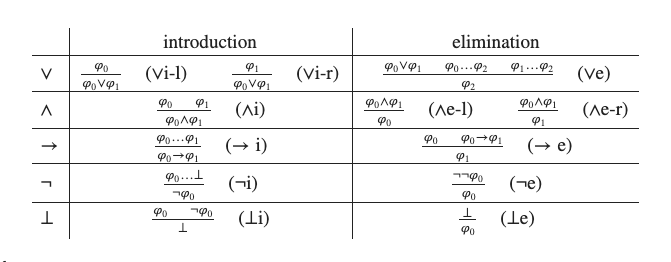
\includegraphics[scale=0.65]{beweisregelnaussagenlogik}\\
    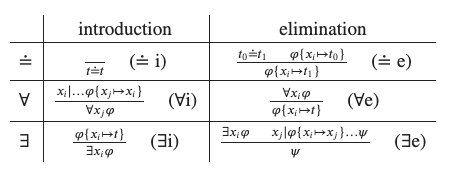
\includegraphics[scale=0.9]{beweisregelnpraedikatenlogik}

    \subsubsection{Korrektheit \& Vollständigkeit}
    \url{---}\\

    \subsection{Resolutionsbeweise}
    \url{---}\\

    \subsubsection{Korrektheit \& Vollständigkeit}
    \url{---}\\

    \subsubsection{Verbindung zwischen Resolution und Logik-Programmierung}
    \url{---}\\

    \section{Kompaktheit}
    \url{---}\\

    \section{Klausuraufgabentypen \& Begriffssammlung}

    \subsection{Aussagenlogik}
    \begin{itemize}
        \item Resultionsbeweis
        \item Modellieren
    \end{itemize}

    \subsection{Prädikatenlogik}
    \begin{itemize}
        \item Ankreuzaufgaben richtig/falsch
        \item Angeben ob Formeln erfüllbar/unerfüllbar/allgmeingültig (mit Beweis)
        \item Formeln für bestimmte Problemstellungen angeben
        \item Äquivalenz von Formeln Beweisen/Widerlegen
        \item Modell für erfüllbare Formlen angeben
        \item Natürlicher Beweis für Allgmeingültigkeit
        \item Resultionsbeweis für Folgerungsbeziehung
    \end{itemize}

    \subsection{Begriffe}
    \begin{multicols}{2}
        \begin{itemize}
            \item Signatur
            \item Struktur
            \item Term
            \item Formel
            \item Relation
            \item BNF
            \item KNF
            \item PNF
            \item Resultionsbeweis
            \item Natürlicher Beweis
            \item Skolemisierung
            \item Unifikation
            \item allgemeinster Unifikator
            \item Vollständigkeit und Korrektheit
            \item Freie Variablen
            \item Scope
            \item Namenskonflikte
            \item Domain
            \item Quantoren / Quantorengesetze
            \item Junktoren
            \item Substitution
            \item Äquivalenz
            \item Koinzidenzlemma
            \item Folgerung
            \item Model
            \item Belegung
            \item Kongruenzlemma
            \item Interpretation von Termen/Formeln
            \item Erfüllbarkeit
            \item Allgmeingültigkeit
        \end{itemize}
    \end{multicols}
    

\end{document}